\section{Feature Based Models of Sentence Salience}

\begin{frame}{Feature Based Models of Sentence Salience}

    Two models for sentence extractive summarization:

    \begin{enumerate}
     \item \textbf{SAP} Sentence salience regression biases an exemplar based
         clustering algorithm (Salience-biased Affinity Propagation Clustering). ~\\~\\
     \item \textbf{L2S} Sentence salience regression with exploration
(learning-to-search)
         for dynamic summary features.
    \end{enumerate}

    ~\\
    Model evaluation on stream summarization task.

\end{frame}

\subsection{Stream Summarization}
\begin{frame}{Stream Summarization}

    {
        \begin{center}
    \includegraphics[scale=.8]{2_feature_based_models_of_salience/image_texs/stream_sum/stream_sum.pdf}
\end{center}
}

Data from TREC Temporal Summarization Track, 2013-2015\\
Query focused crisis monitoring scenario \\
E.g., summarize a stream of news about Hurricane Sandy

\end{frame}

\begin{frame}{Queries and Nuggets}

    TREC data included event queries, i.e. real life natural and man-made
    disasters/crises.\\
    E.g. ``Hurricane Sandy,'' ``Boston Marathon Bombing''\\
~\\
No reference summaries, but reference \textit{nuggets}.
        \begin{tabular}{l}
         \textbf{``hurricane sandy''} \\
        \hline
    $[\textrm{10/23 8:20pm}]$ Sandy strengthened from a tropical depression into\\
    ~~~~~~~~~~~~~~~~~~~~~a tropical storm \\
    $[\textrm{10/23 8:20pm}]$ 2 pm Oct 23 Sandy moving north-northeast at 4 
    knots \\
    $[\textrm{10/23 8:53pm}]$ forecast track uncertain \\
    $[\textrm{10/25 12:20am}]$ In Jamaica damage was extensive\\
\end{tabular}


\end{frame}


\subsection{Features}
\begin{frame}{Features}
  \begin{columns}
      \begin{column}{.5\textwidth}
      \begin{itemize}
        \item Surface Features
        \item Query Features
        \item Language Model Scores
        \item Geographic Relevance (SAP)
        \item Temporal Relevance (SAP)
      \end{itemize}
    \end{column}
    \begin{column}{.5\textwidth}
      \begin{itemize}
        \item Document Frequency (L2S)
        \item Stream Language Model Scores (L2S)
        \item Update Similarity (L2S)
        \item Nugget Probability (L2S)
        \item Single Document Summarization Rankings (L2S)
      \end{itemize}
   \end{column}
  \end{columns}
\end{frame}

\subsection{Salience Biased Affinity Propagation}

\begin{frame}{Salience Biased Affinity Propagation}

 \begin{itemize}
   \item Let $\mathcal{N}(y)$ be the set of nuggets for query $q$.
   \item Salience $y$ of a sentence $s$ is computed: \[y = \max_{n \in \mathcal{N}(q)} 
       \textsc{Similarity}(s,n)\]  where $\textsc{Similarity}(\cdot, \cdot)$
      is the semantic similarity method of Guo and Diab, 20??.
                \item $ \hat{y} = \mathbb{E}_{p(y_*|s_*,S,Y)} \left[y_*\right]$               where $p(y_*|s_*,S, Y)$ is the posterior predictive distribution
                    of a Gaussian Process with training sentences and saliences $S$ and $Y$ respectively.
                \item Predicted saliences $\hat{y}_i$ are then
                    used to bias Affinity Propagation clustering of the sentences. The cluster centers are selected as updates.
 \end{itemize}
\end{frame}

\begin{frame}{Salience Biased Affinity Propagation}
    \center

    \only<1>{ \includegraphics[scale=.8]{images/cluster_anim1.pdf} }
    \only<2>{ \includegraphics[scale=.8]{images/cluster_anim2.pdf} }
    \only<3>{ \includegraphics[scale=.8]{images/cluster_anim3.pdf} }
    \only<4>{ \includegraphics[scale=.8]{images/cluster_anim4.pdf} }
    \only<5>{ \includegraphics[scale=.8]{images/cluster_anim5.pdf} }
    \only<6>{ \includegraphics[scale=.8]{images/cluster_anim6.pdf} }
    \only<7>{ \includegraphics[scale=.8]{images/cluster_anim7.pdf} }

\end{frame}

\begin{frame}
    \frametitle{Experiments}
    
    \begin{itemize}
        \pause
    \item Leave-One-Out evaluation on 21 TREC 2015 Temporal Summarization events
        \pause
        \item 3 events held out for tuning similarity threshold parameters
        \pause
        \item trained salience models for each event
        \pause
        \begin{itemize}
            \item 1000 sentences sampled for each event
            \item at test time, salience prediction is the average of the 
                23 other models
        \end{itemize}
    \end{itemize}
    
\end{frame}

\begin{frame}
    \frametitle{Evaluation Metrics}
    \begin{itemize}
        \pause
        \item ROUGE 
        \pause
        \begin{itemize}
            \item model summary generated by concatenating event nuggets
        \end{itemize}
        \pause
    \item Expected Gain and Comprehensiveness
        $$\mathbb{E}[\mathrm{Gain}] = \frac{|S_n|}{|S|}\;\;\;\;\;\;\;\;\;
            \textrm{Comprehensiveness} = \frac{|S_n|}{|N|}$$
            where \begin{itemize}
                    \pause
            \item[] $S$ is the set of system updates
                    \pause
                \item[] $S_n$ is the set of nuggets mapped to updates in $S$
                    \pause
                \item[] $N$ is the set of nuggets for the event
            \end{itemize}
    \end{itemize}
\end{frame}

\begin{frame}
    \frametitle{Baselines}
    \begin{itemize}
    \item AP+Salience -- full model
    \item AP -- affinity propagation clustering with no salience
    \item HAC -- hierarchical agglomerative clustering
    \item RS -- rank by salience
    \end{itemize}
\end{frame}

\begin{frame}
    \frametitle{ROUGE}
\begin{table}[h]
\centering
% centering table
\begin{tabular}{l c c c}
% creating 10 columns
\multicolumn{4}{c}{ROUGE-1}\\
\hline
\hline
% inserting double-line
$\mathrm{System}$ & $\mathrm{Recall}$ & $\mathrm{Prec.}$ & $\mathrm{F}_1$\\
[0.5ex]
\hline
AP+Salience & $\mathbf{0.282}$ & $\mathbf{0.344}$ & $\mathbf{0.306}$\\
AP          & $0.245$ & $0.285$ & $0.263$ \\
RS          & $0.230$ & $0.271$ & $0.247$ \\
HAC         & $0.169$ & $0.230$ & $0.186$ \\
\hline % inserts single-line
\end{tabular}
~\\[1ex]
~\\
\begin{tabular}{l c c c}
% creating 10 columns
\multicolumn{4}{c}{ROUGE-2}\\
\hline
\hline
% inserting double-line
$\mathrm{System}$ & $\mathrm{Recall}$ & $\mathrm{Prec.}$ & $\mathrm{F}_1$\\[0.5ex]
\hline
\textsc{AP+Salience} & $\mathbf{0.045}$ & $\mathbf{0.056}$ & $\mathbf{0.049}$\\
\textsc{AP}          & $0.033$ & $0.038$ & $0.035$ \\
\textsc{RS}          & $0.031$ & $0.037$ & $0.034$ \\
\textsc{HAC}         & $0.017$ & $0.024$ & $0.019$ \\
\hline % inserts single-line
\end{tabular}
\end{table}
\end{frame}


\begin{frame}
\frametitle{ROUGE-1 over time}
\begin{center}
\includegraphics[]{images/rouge-time.eps}
\end{center}
\end{frame}


\begin{frame}
\frametitle{$\mathbb{E}[\mathrm{Gain}]$ and $\mathrm{Comprehensiveness}$}
\begin{center}
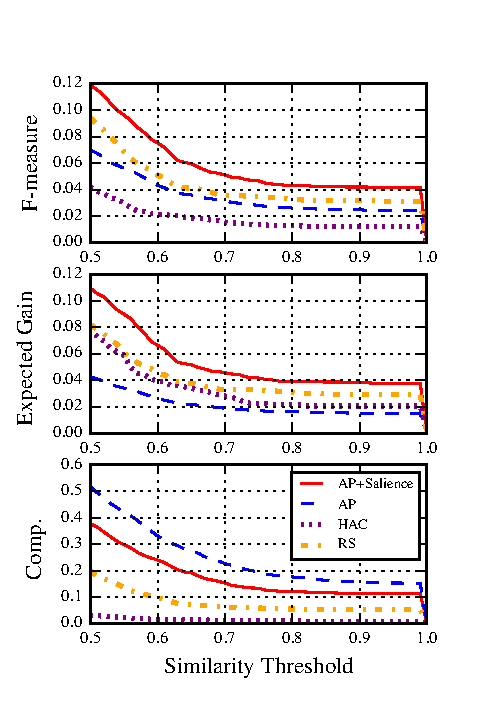
\includegraphics[scale=.7]{images/nuggets-metrics2.eps}
\end{center}
\end{frame}

\subsection{Learning-to-Summarize}


\begin{frame}
\begin{figure}[h]
 \centering
 \begin{tikzpicture}
   \tikzstyle{sent}=[align=left]
   \tikzstyle{doc}=[rectangle,rounded corners,draw=black, very thick]



\node[draw,circle,minimum size=.20cm,inner sep=0pt] (a) at (0,0) {};
\node[draw,circle,minimum size=.20cm,inner sep=0pt] (b) at (.5,0) {};
\node[draw,circle,minimum size=.20cm,inner sep=0pt] (c) at (1,0) {};
\node[draw,circle,minimum size=.20cm,inner sep=0pt] (d) at (1.5,0) {};
\node[draw,circle,minimum size=.20cm,inner sep=0pt] (e) at (2,0) {};
\node[draw,circle,minimum size=.20cm,inner sep=0pt] (f) at (2.5,0) {};
\node[draw,circle,minimum size=.20cm,inner sep=0pt] (g) at (3,0) {};
\node[draw,circle,minimum size=.20cm,inner sep=0pt] (h) at (3.5,0) {};
\node[draw,circle,minimum size=.20cm,inner sep=0pt] (i) at (4,0) {};
\node[draw,circle,minimum size=.20cm,inner sep=0pt] (j) at (4.5,0) {};
\node[draw,circle,minimum size=.20cm,inner sep=0pt] (k) at (5,0) {};
\node[draw,circle,minimum size=.20cm,inner sep=0pt] (l) at (5.5,0) {};
\node[draw,circle,minimum size=.20cm,inner sep=0pt] (m) at (6,0) {};
\node[draw,circle,minimum size=.20cm,inner sep=0pt] (n) at (6.5,0) {};
\node[draw,circle,minimum size=.20cm,inner sep=0pt] (o) at (7,0) {};
\node[draw,circle,minimum size=.20cm,inner sep=0pt] (p) at (7.5,0) {};

\node[draw,circle,minimum size=.20cm,inner sep=0pt] (q) at (.25,.5) {};
\node[draw,circle,minimum size=.20cm,inner sep=0pt] (r) at (1.25,.5) {};
\node[draw,circle,minimum size=.20cm,inner sep=0pt] (s) at (2.25,.5) {};
\node[draw,circle,minimum size=.20cm,inner sep=0pt] (t) at (3.25,.5) {};
\node[draw,circle,minimum size=.20cm,inner sep=0pt] (u) at (4.25,.5) {};
\node[draw,circle,minimum size=.20cm,inner sep=0pt] (v) at (5.25,.5) {};
\node[draw,circle,minimum size=.20cm,inner sep=0pt] (w) at (6.25,.5) {};
\node[draw,circle,minimum size=.20cm,inner sep=0pt] (x) at (7.25,.5) {};

\node[draw,circle,minimum size=.20cm,inner sep=0pt] (y) at (.75,1) {};
\node[draw,circle,minimum size=.20cm,inner sep=0pt] (z) at (2.75,1) {};
\node[draw,circle,minimum size=.20cm,inner sep=0pt] (1) at (4.75,1) {};
\node[draw,circle,minimum size=.20cm,inner sep=0pt] (2) at (6.75,1) {};

\node[draw,circle,minimum size=.20cm,inner sep=0pt] (3) at (1.75,1.5) {};
\node[draw,circle,minimum size=.20cm,inner sep=0pt] (4) at (5.75,1.5) {};

\node[draw,circle,minimum size=.20cm,inner sep=0pt] (5) at (3.75,2.25) {};

\visible<1-17>{
\node[] at ($(x) + (.75,0)$) [] {\footnotesize Sent. 4};
\node[] at ($(x) + (.75,.5)$) [] {\footnotesize Sent. 3};
\node[] at ($(x) + (.75,1)$) [] {\footnotesize Sent. 2};
\node[] at ($(x) + (.75,1.75)$) [] {\footnotesize Sent. 1};
}


\draw[->] (5) -- (3); 
\draw[->] (5) -- (4);


\draw[->] (3) -- (y);
\draw[->] (3) -- (z);

\draw[->] (4) -- (1);
\draw[->] (4) -- (2);


\draw[->] (y) -- (q);
\draw[->] (y) -- (r);

\draw[->] (z) -- (s);
\draw[->] (z) -- (t);

\draw[->] (1) -- (u);
\draw[->] (1) -- (v);

\draw[->] (2) -- (w);
\draw[->] (2) -- (x);




\draw[->] (q) -- (a);
\draw[->] (q) -- (b);

\draw[->] (r) -- (c);
\draw[->] (r) -- (d);

\draw[->] (s) -- (e);
\draw[->] (s) -- (f);

\draw[->] (t) -- (g);
\draw[->] (t) -- (h);

\draw[->] (u) -- (i);
\draw[->] (u) -- (j);

\draw[->] (v) -- (k);
\draw[->] (v) -- (l);

\draw[->] (w) -- (m);
\draw[->] (w) -- (n);

\draw[->] (x) -- (o);
\draw[->] (x) -- (p);

\visible<2>{
\node at ($(5)!0.5!(3)$) [text=green]{$\PlusSmall$};
\node at ($(5)!0.5!(4)$) [text=red]{$\MinusSmall$};
\node at ($(3)!0.5!(y)$) [text=green]{$\PlusSmall$};
\node at ($(3)!0.5!(z)$) [text=red]{$\MinusSmall$};
\node at ($(4)!0.5!(1)$) [text=green]{$\PlusSmall$};
\node at ($(4)!0.5!(2)$) [text=red]{$\MinusSmall$};
\node at ($(y)!0.5!(q)$) [text=green]{$\PlusSmall$};
\node at ($(y)!0.5!(r)$) [text=red]{$\MinusSmall$};
\node at ($(z)!0.5!(s)$) [text=green]{$\PlusSmall$};
\node at ($(z)!0.5!(t)$) [text=red]{$\MinusSmall$};
\node at ($(1)!0.5!(u)$) [text=green]{$\PlusSmall$};
\node at ($(1)!0.5!(v)$) [text=red]{$\MinusSmall$};
\node at ($(2)!0.5!(w)$) [text=green]{$\PlusSmall$};
\node at ($(2)!0.5!(x)$) [text=red]{$\MinusSmall$};
\node at ($(q)!0.5!(a)$) [text=green]{$\PlusSmall$};
\node at ($(q)!0.5!(b)$) [text=red]{$\MinusSmall$};
\node at ($(r)!0.5!(c)$) [text=green]{$\PlusSmall$};
\node at ($(r)!0.5!(d)$) [text=red]{$\MinusSmall$};
\node at ($(s)!0.5!(e)$) [text=green]{$\PlusSmall$};
\node at ($(s)!0.5!(f)$) [text=red]{$\MinusSmall$};
\node at ($(t)!0.5!(g)$) [text=green]{$\PlusSmall$};
\node at ($(t)!0.5!(h)$) [text=red]{$\MinusSmall$};
\node at ($(u)!0.5!(i)$) [text=green]{$\PlusSmall$};
\node at ($(u)!0.5!(j)$) [text=red]{$\MinusSmall$};
\node at ($(v)!0.5!(k)$) [text=green]{$\PlusSmall$};
\node at ($(v)!0.5!(l)$) [text=red]{$\MinusSmall$};
\node at ($(w)!0.5!(m)$) [text=green]{$\PlusSmall$};
\node at ($(w)!0.5!(n)$) [text=red]{$\MinusSmall$};
\node at ($(x)!0.5!(o)$) [text=green]{$\PlusSmall$};
\node at ($(x)!0.5!(p)$) [text=red]{$\MinusSmall$};
};

\visible<4-7>{
\draw[-,color=orange,very thick,dashed,line width=0.1cm] (5) -- (3); 
}
\visible<5-7>{
\draw[-,color=orange,very thick,dashed,line width=0.1cm] (3) -- (z); 
}
\visible<6-7>{
\draw[-,color=orange,very thick,dashed,line width=0.1cm] (z) -- (s); 
}
\visible<7>{
\draw[-,color=orange,very thick,dashed,line width=0.1cm] (s) -- (e); 
}
\visible<9-12>{
\draw[-,color=orange,very thick,dashed,line width=0.1cm] (5) -- (3); 
}
\visible<10-12>{
\draw[-,color=orange,very thick,dashed,line width=0.1cm] (3) -- (z); 
}
\visible<11-12>{
\draw[-,color=orange,very thick,dashed,line width=0.1cm] (z) -- (s); 
}
\visible<12>{
\draw[-,color=orange,very thick,dashed,line width=0.1cm] (s) -- (e); 
}




\visible<14-17>{
\draw[-,color=purple,very thick,dashed,line width=0.1cm] (5) -- (4); 
}
\visible<15-17>{
\draw[-,color=purple,very thick,dashed,line width=0.1cm] (4) -- (2); 
}
\visible<16-17>{
\draw[-,color=purple,very thick,dashed,line width=0.1cm] (2) -- (w); 
}
\visible<17>{
\draw[-,color=purple,very thick,dashed,line width=0.1cm] (w) -- (n); 
}



\visible<3>{
  \node[draw,circle,minimum size=.45cm,inner sep=0pt,dashed,thick] at (5) {}; 
}
\visible<4>{
  \node[draw,circle,minimum size=.45cm,inner sep=0pt,dashed,thick] at (3) {}; 
}
\visible<5>{
  \node[draw,circle,minimum size=.45cm,inner sep=0pt,dashed,thick] at (z) {}; 
}
\visible<6>{
  \node[draw,circle,minimum size=.45cm,inner sep=0pt,dashed,thick] at (s) {}; 
}
\visible<7>{
  \node[draw,circle,minimum size=.45cm,inner sep=0pt,dashed,thick] at (e) {}; 
}
\visible<8>{
  \node[draw,circle,minimum size=.45cm,inner sep=0pt,dashed,thick] at (5) {}; 
}
\visible<9>{
  \node[draw,circle,minimum size=.45cm,inner sep=0pt,dashed,thick] at (3) {}; 
}
\visible<10>{
  \node[draw,circle,minimum size=.45cm,inner sep=0pt,dashed,thick] at (z) {}; 
}
\visible<11>{
  \node[draw,circle,minimum size=.45cm,inner sep=0pt,dashed,thick] at (s) {}; 
}
\visible<12>{
  \node[draw,circle,minimum size=.45cm,inner sep=0pt,dashed,thick] at (e) {}; 
}


\visible<13>{
  \node[draw,circle,minimum size=.45cm,inner sep=0pt,dashed,thick] at (5) {}; 
}
\visible<14>{
  \node[draw,circle,minimum size=.45cm,inner sep=0pt,dashed,thick] at (4) {}; 
}
\visible<15>{
  \node[draw,circle,minimum size=.45cm,inner sep=0pt,dashed,thick] at (2) {}; 
}
\visible<16>{
  \node[draw,circle,minimum size=.45cm,inner sep=0pt,dashed,thick] at (w) {}; 
}
\visible<17>{
  \node[draw,circle,minimum size=.45cm,inner sep=0pt,dashed,thick] at (n) {}; 
}


%\visible<-4>{
   \visible<4-7,9-17>{
       \node[sent,left] at (5.5, -1) {\fontsize{7}{11}\selectfont 
       {\large\{} ~~~~~~~~~~ ``explosions'', ~~~~~~~~~~ ``finish line 
           Marathon'' 
       {\large\}}}; 
       \node at (.2,-1) [rectangle,fill=yellow,text=orange,rounded corners] 
       {\fontsize{6}{8}\selectfont \textbf{A}};

       \node at (2.4,-1) [rectangle,fill=yellow,text=blue,rounded corners] 
       {\fontsize{6}{8}\selectfont \textbf{B}};
   }
   \visible<6-7,11-17>{
       \node[sent,left] at (5.5, -1.5) 
       {\fontsize{7}{11}\selectfont 
       {\large\{} ~~~~~~~~~~ ``two bombs,'' ~~~~~~~~~~ ``finish line 
           Marathon'' 
           {\large\}}};
       \node at (.2,-1.5) [rectangle,fill=yellow,text=red,rounded corners] 
       {\fontsize{6}{8}\selectfont \textbf{C}};
       
       \node at (2.4,-1.5) [rectangle,fill=yellow,text=blue, rounded corners] 
       {\fontsize{6}{8}\selectfont \textbf{B}};
   }
   \visible<7,12-17>{
   \node[sent,left] at (5.5, -2) 
   {\fontsize{7}{11}\selectfont {\large\{} ~~~~~~~~~~ ``Many injured''
       {\large\}}};
       \node at (3.1,-2) [rectangle,fill=yellow,text=green!50,
                           rounded corners] 
       {\fontsize{6}{8}\selectfont \textbf{D}};
   }



   \visible<3-17>{
   \draw[-,thick,rounded corners] (-.5,-1) -- (-.5, -.65) -- (5.5, -.65)
       -- (5.5, -2.45) -- (-.5, -2.45) -- (-.5,-1.);
  \node (O) at (1.7,-2.55) [fill=orange!20,rounded corners] { Oracle Summary};
   }
   \visible<8-12>{
       \node (ARRAY) at ($(O)+(6,-1.25)$) [align=center] 
       {$\phi(s) \triangleq $ feature \\function of state $s$};
       \node (ARRAY) at ($(O)+(0,-1.25)$) [] 
   {\begin{minipage}{3cm} 
           $X = \left[ \begin{array}{c} 
                   \visible<9-12>{\phi(s_1)} \\ 
                   \visible<10-12>{\phi(s_2)} \\ 
                   \visible<11-12>{\phi(s_3)} \\ 
                   \visible<12-12>{\phi(s_4)} \\ 
   \end{array} \right]$ \end{minipage} };
   \node (ARRAY2) at ($(ARRAY)+(3,0)$) [] 
   {\begin{minipage}{3cm} 
           $y = \left[ \begin{array}{c} 
                   \visible<9-12>{select} \\ 
                   \visible<10-12>{skip} \\ 
                   \visible<11-12>{select} \\ 
                   \visible<12-12>{select} \\ 
   \end{array} \right]$ \end{minipage} };
  % {$\begin{array}{l} \phi(s_0) \\ \phi(s_1) \\ \phi(s_2) \end{array}$};
   }
   \visible<8-17>{
   \node at ($(O)+(6,1)$) [rounded corners,fill=purple!20,align=center] 
       {Learned Policy: \\ Naive \\Classification \\ Model};
   }

   \visible<18-19>{
\begin{pgflowlevelscope}{\pgftransformscale{0.25}}
\draw [decorate,decoration={brace,amplitude=16pt,mirror,raise=4pt,},
       line width=.1cm,yshift=0pt]
($(31,-.5)$) -- ($(31,4.25)+(0,0)$) node [black,midway,xshift=0.8cm] {};
\end{pgflowlevelscope}
\begin{pgflowlevelscope}{\pgftransformscale{0.25}}
\draw [decorate,decoration={brace,amplitude=16pt,mirror,raise=4pt,},
       line width=.1cm,yshift=0pt]
($(31,6)$) -- ($(31,9.5)+(0,0)$) node [black,midway,xshift=0.8cm] {};
\end{pgflowlevelscope}
\node[] at ($(x) + (1.6,1.45)$) [align=center] 
    {\footnotesize Roll-in: $\hat{\pi}$};
}
   
\visible<18>{
\node[] at ($(x) + (1.6,0)$) [align=center] 
    {\footnotesize Roll-out: $\pi^*$};
}
\visible<19>{
\node[] at ($(x) + (1.6,0)$) [align=center] 
{\footnotesize Roll-out: $\hat{\pi}$};
}

\visible<19>{
\draw[-,color=purple,very thick,dashed,line width=0.1cm] (5) -- (4); 
\draw[-,black=purple,very thick,dashed,line width=0.1cm] (4) -- (2); 
\draw[-,black=purple,very thick,dashed,line width=0.1cm] (4) -- (1); 
\draw[-,color=purple,very thick,dashed,line width=0.1cm] (1) -- (v); 
\draw[-,color=purple,very thick,dashed,line width=0.1cm] (v) -- (l); 
\draw[-,color=purple,very thick,dashed,line width=0.1cm] (2) -- (w); 
\draw[-,color=purple,very thick,dashed,line width=0.1cm] (w) -- (n); 
  \node[draw,circle,minimum size=.45cm,inner sep=0pt,dashed,thick] at (l) {}; 
  \node[draw,circle,minimum size=.45cm,inner sep=0pt,dashed,thick] at (n) {}; 
  \node at ($(a)+(0,-.75)$) [] {$Cost$:};
  \draw[-] ($(l)+(-.5,-1)$) -- ($(l)+(.5,-1)$) 
   node[midway,rectangle,text height=.25cm,fill=red!40,yshift=.26cm] (xx) {};
  \draw[-] ($(n)+(-.5,-1)$) -- ($(n)+(.5,-1)$) 
   node[midway,rectangle,text height=.15cm,fill=red!40,yshift=.21cm] (xx) {};
   \node at ($(l)+(-1.75,-1)$) [] {$c(s_2,select)$};
   \node at ($(n)+(1.75,-1)$) [] {$c(s_2,skip)$};

}


   \visible<8-12,18-26>{
       \node at ($(5)+(.5,0)$) [] {$s_1$};
   }
   \visible<18-19,21-26>{
       \node at ($(4)+(.5,0)$) [] {$s_2$};
   }

   \visible<22-26>{
       \node at ($(2)+(.5,0)$) [] {$s_3$};
   }
   \visible<23-26>{
       \node at ($(w)+(-.5,0)$) [] {$s_4$};
   }
   \visible<9-12>{
       \node at ($(3)+(-.5,.25)$) [] {$s_2$};
   }
   \visible<10-12>{
       \node at ($(z)+(.5,.25)$) [] {$s_3$};
   }
   \visible<11-12>{
       \node at ($(s)+(-.5,.25)$) [] {$s_4$};
   }
   \visible<16-17>{    
   \node[sent,left] at (5.5, -3.5) 
   {\fontsize{7}{11}\selectfont 
   {\large\{} ~~~~~~~~~~ ``two bombs,'' ~~~~~~~~~~ ``finish line Marathon'' 
       {\large\}}};
   \node at (.2,-3.5) [rectangle,fill=yellow,text=red,rounded corners] 
   {\fontsize{6}{8}\selectfont \textbf{C}};
   
   \node at (2.4,-3.5) [rectangle,fill=yellow,text=blue,rounded corners] 
   {\fontsize{6}{8}\selectfont \textbf{B}};
   }
\visible<13-17>{
   \draw[-,thick,rounded corners] (-.5,-3.5) -- (-.5, -3.15) -- (5.5, -3.15)
       -- (5.5, -3.9) -- (-.5, -3.9) -- (-.5,-3.5);
   \node at (1.7,-4.05) [fill=purple!20,rounded corners] { Predicted Summary};
}

%\visible<20>{
%
%   %\node at ($(5)+(-3.2,.1)$) [rectangle,fill=orange!20,rounded corners] 
%   %        {\Large Oracle Rollout};
%
%  \node[draw,circle,minimum size=.45cm,inner sep=0pt,dashed,thick] at (5) {}; 
%
%  \draw[-,color=black,very thick,dashed,line width=0.1cm] (5) -- (3); 
%  \draw[-,color=black,very thick,dashed,line width=0.1cm] (5) -- (4); 
%}
%\visible<20>{
%   \draw[-,color=orange,very thick,dashed,line width=0.1cm] (3) -- (z); 
%   \draw[-,color=orange,very thick,dashed,line width=0.1cm] (z) -- (s); 
%   \draw[-,color=orange,very thick,dashed,line width=0.1cm] (s) -- (e); 
%
%  \draw[-,color=orange,very thick,dashed,line width=0.1cm] (4) -- (2); 
%  \draw[-,color=orange,very thick,dashed,line width=0.1cm] (2) -- (w); 
%  \draw[-,color=orange,very thick,dashed,line width=0.1cm] (w) -- (m); 
%  \node[draw,circle,minimum size=.45cm,inner sep=0pt,dashed,thick] at (e) {}; 
%  \node[draw,circle,minimum size=.45cm,inner sep=0pt,dashed,thick] at (m) {}; 
%}
%\visible<20>{
%  \node at ($(a)+(0,-.75)$) [] {$Cost$:};
%  \draw[-] ($(e)+(-.5,-1)$) -- ($(e)+(.5,-1)$) 
%   node[midway,rectangle,text height=.01cm,fill=red!40,yshift=.14cm] (xx) {};
%  \draw[-] ($(m)+(-.5,-1)$) -- ($(m)+(.5,-1)$) 
%   node[midway,rectangle,text height=.15cm,fill=red!40,yshift=.21cm] (xx) {};
%   \node at ($(e)+(1.75,-1)$) [] {$c(s_0,select)$};
%   \node at ($(m)+(1.75,-1)$) [] {$c(s_0,skip)$};
%}  

\visible<18>{

  \node[draw,circle,minimum size=.45cm,inner sep=0pt,dashed,thick] at (4) {}; 
  \draw[-,color=purple,very thick,dashed,line width=0.1cm] (5) -- (4); 
  \draw[-,color=orange,very thick,dashed,line width=0.1cm] (1) -- (u); 
  \draw[-,color=orange,very thick,dashed,line width=0.1cm] (u) -- (i); 

  \draw[-,color=black,very thick,dashed,line width=0.1cm] (4) -- (2); 
  \draw[-,color=black,very thick,dashed,line width=0.1cm] (4) -- (1); 
  \draw[-,color=orange,very thick,dashed,line width=0.1cm] (2) -- (w); 
  \draw[-,color=orange,very thick,dashed,line width=0.1cm] (w) -- (m); 

  \node at ($(a)+(0,-.75)$) [] {$Cost$:};
  \draw[-] ($(i)+(-.5,-1)$) -- ($(i)+(.5,-1)$) 
   node[midway,rectangle,text height=.25cm,fill=red!40,yshift=.26cm] (xx) {};
  \draw[-] ($(m)+(-.5,-1)$) -- ($(m)+(.5,-1)$) 
   node[midway,rectangle,text height=.15cm,fill=red!40,yshift=.21cm] (xx) {};
   \node at ($(i)+(-1.75,-1)$) [] {$c(s_2,select)$};
   \node at ($(m)+(1.75,-1)$) [] {$c(s_2,skip)$};
  
  \node[draw,circle,minimum size=.45cm,inner sep=0pt,dashed,thick] at (i) {}; 
  \node[draw,circle,minimum size=.45cm,inner sep=0pt,dashed,thick] at (m) {}; 
}   
%
%\visible<20>{
%
%  \node[draw,circle,minimum size=.45cm,inner sep=0pt,dashed,thick] at (2) {};
%  \draw[-,color=purple,very thick,dashed,line width=0.1cm] (5) -- (4); 
%  \draw[-,color=purple,very thick,dashed,line width=0.1cm] (4) -- (2); 
%  \draw[-,color=black,very thick,dashed,line width=0.1cm] (2) -- (w); 
%  \draw[-,color=black,very thick,dashed,line width=0.1cm] (2) -- (x); 
%  \draw[-,color=orange,very thick,dashed,line width=0.1cm] (w) -- (m); 
%  \draw[-,color=orange,very thick,dashed,line width=0.1cm] (x) -- (o); 
%
%  \node at ($(a)+(0,-.75)$) [] {$Cost$:};
%  \draw[-] ($(o)+(-.5,-1)$) -- ($(o)+(.5,-1)$) 
%   node[midway,rectangle,text height=.25cm,fill=red!40,yshift=.26cm] (xx) {};
%  \draw[-] ($(m)+(-.5,-1)$) -- ($(m)+(.5,-1)$) 
%   node[midway,rectangle,text height=.15cm,fill=red!40,yshift=.21cm] (xx) {};
%   \node at ($(m)+(-1.75,-1)$) [] {$c(s_2,select)$};
%   \node at ($(o)+(1.75,-1)$) [] {$c(s_2,skip)$};
%  
%  \node[draw,circle,minimum size=.45cm,inner sep=0pt,dashed,thick] at (m) {}; 
%  \node[draw,circle,minimum size=.45cm,inner sep=0pt,dashed,thick] at (o) {}; 
%}
%\visible<21-22>{
%
%  \node[draw,circle,minimum size=.45cm,inner sep=0pt,dashed,thick] at (w) {}; 
%
%  \draw[-,color=purple,very thick,dashed,line width=0.1cm] (5) -- (4); 
%  \draw[-,color=purple,very thick,dashed,line width=0.1cm] (4) -- (2); 
%  \draw[-,color=purple,very thick,dashed,line width=0.1cm] (2) -- (w); 
%  \draw[-,color=black,very thick,dashed,line width=0.1cm] (w) -- (m); 
%  \draw[-,color=black,very thick,dashed,line width=0.1cm] (w) -- (n); 
%
%  \node at ($(a)+(0,-.75)$) [] {$Cost$:};
%  \draw[-] ($(n)+(-.5,-1)$) -- ($(n)+(.5,-1)$) 
%   node[midway,rectangle,text height=.075cm,fill=red!40,yshift=.175cm] (xx) {};
%  \draw[-] ($(m)+(-.5,-1)$) -- ($(m)+(.5,-1)$) 
%   node[midway,rectangle,text height=.15cm,fill=red!40,yshift=.215cm] (xx) {};
%   \node at ($(m)+(-1.75,-1)$) [] {$c(s_3,select)$};
%   \node at ($(n)+(1.75,-1)$) [] {$c(s_3,skip)$};
%  
%  \node[draw,circle,minimum size=.45cm,inner sep=0pt,dashed,thick] at (m) {}; 
%  \node[draw,circle,minimum size=.45cm,inner sep=0pt,dashed,thick] at (n) {}; 
%}
%
   \visible<20-26>{
       \node (ARRAY) at ($(e)+(-1,-2.2)$) [] 
   {\begin{minipage}{3cm}\scriptsize
           $X = \left[ \begin{array}{c} 
                   \visible<20-26>{\phi(s_1)} \\ 
                   \visible<21-26>{\phi(s_2)} \\ 
                   \visible<22-26>{\phi(s_3)} \\ 
                   \visible<23-26>{\phi(s_4)} \\ 
   \end{array} \right]$ \end{minipage} };
   \node (ARRAY2) at ($(ARRAY)+(3,0)$) [draw] 
   {\begin{minipage}{3.75cm}\scriptsize
           $y_{select} = \left[ \begin{array}{c} 
                   \visible<20-26>{c(s_1,select)} \\ 
                   \visible<21-26>{c(s_2, select)} \\ 
                   \visible<22-26>{c(s_3, select)} \\ 
                   \visible<23-26>{c(s_4, select)} \\ 
   \end{array} \right]$ \end{minipage} };
   \node (ARRAY3) at ($(ARRAY2)+(4,0)$) [draw] 
   {\begin{minipage}{3.5cm}\scriptsize 
           $y_{skip} = \left[ \begin{array}{c} 
                   \visible<20-26>{c(s_1, skip)} \\ 
                   \visible<21-26>{c(s_2, skip)} \\ 
                   \visible<22-26>{c(s_3, skip)} \\ 
                   \visible<23-26>{c(s_4, skip)} \\ 
   \end{array} \right]$ \end{minipage} };
  }
   \visible<24-26>{
   \node at ($(ARRAY2)+(-2.5,-1.6)$) [align=center] 
   {$\hat{c}(s,select) = w_{select} \cdot \phi(s)$  \\
    $\hat{c}(s,skip) = w_{skip} \cdot \phi(s)$};
    }
   \visible<25-26>{
   \node (LP) at ($(i)+(3,-4.25)$) 
   [align=center,rounded corners,fill=purple!20] 
   {Learned Policy: \\
       $\displaystyle \hat{\pi}(s) = 
       \argmin_{a \in \{select,skip\}} \hat{c}(s,a)$};


   }


\visible<20>{
\begin{pgflowlevelscope}{\pgftransformscale{0.25}}
\draw [decorate,decoration={brace,amplitude=16pt,mirror,raise=4pt,},
       line width=.1cm,yshift=0pt]
($(31,-.5)$) -- ($(31,6)+(0,0)$) node [black,midway,xshift=0.8cm] {};
\end{pgflowlevelscope}
\node[] at ($(x) + (1.5,.2)$) [align=center] 
    {\footnotesize Roll-out: $\hat{\pi}$};
}
\visible<20>{

  \node[draw,circle,minimum size=.45cm,inner sep=0pt,dashed,thick] at (5) {}; 

  \draw[-,color=black,very thick,dashed,line width=0.1cm] (5) -- (3); 
  \draw[-,color=black,very thick,dashed,line width=0.1cm] (5) -- (4); 
   \draw[-,color=purple,very thick,dashed,line width=0.1cm] (3) -- (z); 
   \draw[-,color=purple,very thick,dashed,line width=0.1cm] (z) -- (t); 
   \draw[-,color=purple,very thick,dashed,line width=0.1cm] (t) -- (g); 



\draw[-,color=purple,very thick,dashed,line width=0.1cm] (4) -- (2); 
\draw[-,color=purple,very thick,dashed,line width=0.1cm] (2) -- (w); 
\draw[-,color=purple,very thick,dashed,line width=0.1cm] (w) -- (n); 

  \node at ($(a)+(0,-.75)$) [] {$Cost$:};
  \draw[-] ($(g)+(-.5,-1)$) -- ($(g)+(.5,-1)$) 
   node[midway,rectangle,text height=.01cm,fill=red!40,yshift=.14cm] (xx) {};
  \draw[-] ($(n)+(-.5,-1)$) -- ($(n)+(.5,-1)$) 
   node[midway,rectangle,text height=.15cm,fill=red!40,yshift=.21cm] (xx) {};
   \node at ($(g)+(-1.5,-1)$) [] {$c(s_1,select)$};
   \node at ($(n)+(1.5,-1)$) [] {$c(s_1, skip)$};
  \node[draw,circle,minimum size=.45cm,inner sep=0pt,dashed,thick] at (g) {}; 
  \node[draw,circle,minimum size=.45cm,inner sep=0pt,dashed,thick] at (n) {}; 
   
}


\visible<21>{
\begin{pgflowlevelscope}{\pgftransformscale{0.25}}
\draw [decorate,decoration={brace,amplitude=16pt,mirror,raise=4pt,},
       line width=.1cm,yshift=0pt]
($(31,-.5)$) -- ($(31,4.25)+(0,0)$) node [black,midway,xshift=0.8cm] {};
\end{pgflowlevelscope}
\node[] at ($(x) + (1.6,0)$) [align=center] 
    {\footnotesize Roll-out: $\pi^*$};
\begin{pgflowlevelscope}{\pgftransformscale{0.25}}
\draw [decorate,decoration={brace,amplitude=16pt,mirror,raise=4pt,},
       line width=.1cm,yshift=0pt]
($(31,6)$) -- ($(31,9.5)+(0,0)$) node [black,midway,xshift=0.8cm] {};
\end{pgflowlevelscope}
\node[] at ($(x) + (1.6,1.45)$) [align=center] 
    {\footnotesize Roll-in: $\hat{\pi}$};
}
\visible<21>{

  \node[draw,circle,minimum size=.45cm,inner sep=0pt,dashed,thick] at (4) {}; 
  \draw[-,color=purple,very thick,dashed,line width=0.1cm] (5) -- (4); 
  \draw[-,color=orange,very thick,dashed,line width=0.1cm] (1) -- (u); 
  \draw[-,color=orange,very thick,dashed,line width=0.1cm] (u) -- (i); 

  \draw[-,color=black,very thick,dashed,line width=0.1cm] (4) -- (2); 
  \draw[-,color=black,very thick,dashed,line width=0.1cm] (4) -- (1); 
  \draw[-,color=orange,very thick,dashed,line width=0.1cm] (2) -- (w); 
  \draw[-,color=orange,very thick,dashed,line width=0.1cm] (w) -- (m); 

  \node at ($(a)+(0,-.75)$) [] {$Cost$:};
  \draw[-] ($(i)+(-.5,-1)$) -- ($(i)+(.5,-1)$) 
   node[midway,rectangle,text height=.25cm,fill=red!40,yshift=.26cm] (xx) {};
  \draw[-] ($(m)+(-.5,-1)$) -- ($(m)+(.5,-1)$) 
   node[midway,rectangle,text height=.15cm,fill=red!40,yshift=.21cm] (xx) {};
   \node at ($(i)+(-1.5,-1)$) [] {$c(s_2, select)$};
   \node at ($(m)+(1.5,-1)$) [] {$c(s_2, skip)$};
  
  \node[draw,circle,minimum size=.45cm,inner sep=0pt,dashed,thick] at (i) {}; 
  \node[draw,circle,minimum size=.45cm,inner sep=0pt,dashed,thick] at (m) {}; 
}
\visible<22>{
\begin{pgflowlevelscope}{\pgftransformscale{0.25}}
\draw [decorate,decoration={brace,amplitude=16pt,mirror,raise=4pt,},
       line width=.1cm,yshift=0pt]
($(31,-.5)$) -- ($(31,2.2)+(0,0)$) node [black,midway,xshift=0.8cm] {};
\end{pgflowlevelscope}
\node[] at ($(x) + (1.6,-.25)$) [align=center] 
    {\footnotesize Roll-out: $\hat{\pi}$};
\begin{pgflowlevelscope}{\pgftransformscale{0.25}}
\draw [decorate,decoration={brace,amplitude=16pt,mirror,raise=4pt,},
       line width=.1cm,yshift=0pt]
($(31,3.75)$) -- ($(31,9.5)+(0,0)$) node [black,midway,xshift=0.8cm] {};
\end{pgflowlevelscope}
\node[] at ($(x) + (1.6,1.15)$) [align=center] 
    {\footnotesize Roll-in: $\hat{\pi}$};
}
\visible<22>{

  \node[draw,circle,minimum size=.45cm,inner sep=0pt,dashed,thick] at (2) {}; 
  \draw[-,color=purple,very thick,dashed,line width=0.1cm] (5) -- (4); 
  \draw[-,color=purple,very thick,dashed,line width=0.1cm] (4) -- (2); 

  \draw[-,color=black,very thick,dashed,line width=0.1cm] (2) -- (w); 
  \draw[-,color=purple,very thick,dashed,line width=0.1cm] (w) -- (n); 

  \draw[-,color=black,very thick,dashed,line width=0.1cm] (2) -- (x); 
  \draw[-,color=purple,very thick,dashed,line width=0.1cm] (x) -- (p); 


%   \draw[-,color=black,very thick,dashed,line width=0.1cm] (4) -- (1); 
%   \draw[-,color=purple,very thick,dashed,line width=0.1cm] (v) -- (k); 

  \node at ($(a)+(0,-.75)$) [] {$Cost$:};
  \draw[-] ($(p)+(-.5,-1)$) -- ($(p)+(.5,-1)$) 
   node[midway,rectangle,text height=.25cm,fill=red!40,yshift=.25cm] (xx) {};


  \draw[-] ($(n)+(-.5,-1)$) -- ($(n)+(.5,-1)$) 
   node[midway,rectangle,text height=.15cm,fill=red!40,yshift=.21cm] (xx) {};
   \node at ($(n)+(-1.5,-1)$) [] {$c(s_3,select)$};
   \node at ($(p)+(1.5,-1)$) [] {$c(s_3,skip)$};
  \node[draw,circle,minimum size=.45cm,inner sep=0pt,dashed,thick] at (p) {}; 
  \node[draw,circle,minimum size=.45cm,inner sep=0pt,dashed,thick] at (n) {}; 
   
}




\visible<23>{
\begin{pgflowlevelscope}{\pgftransformscale{0.25}}
\draw [decorate,decoration={brace,amplitude=16pt,mirror,raise=4pt,},
       line width=.1cm,yshift=0pt]
($(31,2)$) -- ($(31,9.5)+(0,0)$) node [black,midway,xshift=0.8cm] {};
\end{pgflowlevelscope}
\node[] at ($(x) + (1.6,1)$) [align=center] 
    {\footnotesize Roll-in: $\hat{\pi}$};
}
\visible<23>{

  \node[draw,circle,minimum size=.45cm,inner sep=0pt,dashed,thick] at (w) {}; 

  \draw[-,color=purple,very thick,dashed,line width=0.1cm] (5) -- (4); 
  \draw[-,color=purple,very thick,dashed,line width=0.1cm] (4) -- (2); 
  \draw[-,color=purple,very thick,dashed,line width=0.1cm] (2) -- (w); 
  \draw[-,color=black,very thick,dashed,line width=0.1cm] (w) -- (m); 
  \draw[-,color=black,very thick,dashed,line width=0.1cm] (w) -- (n); 

  \node at ($(a)+(0,-.75)$) [] {$Cost$:};
  \draw[-] ($(n)+(-.5,-1)$) -- ($(n)+(.5,-1)$) 
   node[midway,rectangle,text height=.075cm,fill=red!40,yshift=.175cm] (xx) {};
  \draw[-] ($(m)+(-.5,-1)$) -- ($(m)+(.5,-1)$) 
   node[midway,rectangle,text height=.15cm,fill=red!40,yshift=.215cm] (xx) {};
   \node at ($(m)+(-1.5,-1)$) [] {$c(s_4, select)$};
   \node at ($(n)+(1.5,-1)$) [] {$c(s_4, skip)$};
  
  \node[draw,circle,minimum size=.45cm,inner sep=0pt,dashed,thick] at (m) {}; 
  \node[draw,circle,minimum size=.45cm,inner sep=0pt,dashed,thick] at (n) {}; 
}
\visible<26>{
       \node at ($(i)+(0,0)$) 
           [align=center,rounded corners,fill=purple!20] 
       {Locally Optimal Learning to Search (LOLS)\footnotemark \\
           Roll-in: $\hat{\pi}$\\
       Roll-out: Randomly choose $\pi^*$ or $\hat{\pi}$}; 
   
       \node at ($(i)+(0,3)$)  {\begin{minipage}{9cm} \tiny
    $~^1$ Kai-Wei Chang, Akshay Krishnamurthy, Alekh Agarwal, Hal Daume, and John 
    Langford. Learning to search better than your teacher. In 
\emph{Proceedings of the ICML-15} \end{minipage}};
   }
\end{tikzpicture}
\end{figure}
\end{frame}

\begin{frame}{Results}
\centering
\only<1>{\includegraphics[scale=.45]{images/section2/uresults1.pdf}}
\only<2>{\includegraphics[scale=.45]{images/section2/uresults2.pdf}}
\only<3>{\includegraphics[scale=.45]{images/section2/uresults3.pdf}}
\only<4>{\includegraphics[scale=.45]{images/section2/uresults4.pdf}}
\only<5>{\includegraphics[scale=.45]{images/section2/uresults5.pdf}}

\end{frame}

\begin{frame}{Latency Penalized Results}
\centering
\only<1>{\includegraphics[scale=.45]{images/section2/results1.pdf}}
\only<2>{\includegraphics[scale=.45]{images/section2/results2.pdf}}
\only<3>{\includegraphics[scale=.45]{images/section2/results3.pdf}}
\only<4>{\includegraphics[scale=.45]{images/section2/results4.pdf}}
\only<5>{\includegraphics[scale=.45]{images/section2/results5.pdf}}

\end{frame}

\begin{frame}{Latency Penalized Results (First Sentence Only)}
\centering
\only<1>{\includegraphics[scale=.45]{images/section2/fsresults1.pdf}}
\only<2>{\includegraphics[scale=.45]{images/section2/fsresults2.pdf}}

\end{frame}

\begin{frame}{Feature Based Models of Sentence Salience: Takeaways}
  this was important because

\end{frame}
